\section{LVLMs: Khi Mô hình Ngôn ngữ Bắt đầu ''Nhìn''}
\label{sec:lvlms}

\subsection{Khái niệm: Hợp nhất Thị giác và Ngôn ngữ}
\label{subsec:lvlm_concept}
Sự ra đời của CLIP đã chứng minh rằng có thể xây dựng một không gian biểu diễn chung cho hình ảnh và văn bản. Tuy nhiên, CLIP chủ yếu là một mô hình "đối sánh" (matching model); nó có thể cho biết một bức ảnh và một câu văn có khớp với nhau hay không, nhưng nó không thể "trò chuyện" về bức ảnh đó.

Đây chính là bước nhảy vọt mà các \textbf{Mô hình Ngôn ngữ-Thị giác Lớn (Large Vision-Language Models - LVLMs)} mang lại. LVLMs, đôi khi còn được gọi là Mô hình Đa phương thức Lớn (Large Multimodal Models - LMMs), là thế hệ tiếp theo của AI, kết hợp sức mạnh biểu diễn của các mô hình thị giác nền tảng (foundation vision models) với khả năng lý luận và sinh ngôn ngữ của các Mô hình Ngôn ngữ Lớn (Large Language Models - LLMs).

Thay vì chỉ đưa ra một nhãn lớp hay một bounding box, LVLMs có khả năng:
\begin{itemize}
	\item \textbf{Trả lời câu hỏi về hình ảnh (Visual Question Answering - VQA):} Người dùng có thể đặt các câu hỏi phức tạp về nội dung, bối cảnh, và các mối quan hệ trong một bức ảnh.
	\item \textbf{Sinh chú thích chi tiết (Dense Captioning):} Mô tả một cách chi tiết những gì đang diễn ra trong ảnh.
	\item \textbf{Thực hiện lý luận thị giác (Visual Reasoning):} Suy luận về các khái niệm trừu tượng, nhân quả, hoặc logic dựa trên thông tin thị giác.
	\item \textbf{Tương tác đa lượt (Multi-turn Dialogue):} Tham gia vào một cuộc trò chuyện về một hoặc nhiều hình ảnh.
\end{itemize}
Sự phát triển của LVLMs đánh dấu một sự chuyển dịch quan trọng từ các mô hình thị giác chuyên biệt sang các \textbf{hệ thống AI tổng quát (general-purpose AI systems)} có khả năng nhận thức và tương tác với thế giới một cách đa chiều.

\subsection{Kiến trúc chung của LVLMs}
\label{subsec:lvlm_general_architecture}
Hầu hết các LVLMs hiện đại đều chia sẻ một kiến trúc chung gồm ba thành phần chính:

\begin{enumerate}
	\item \textbf{Bộ mã hóa Thị giác (Vision Encoder):} Một mô hình thị giác nền tảng mạnh mẽ (thường là một ViT được huấn luyện trước như CLIP hoặc DINOv2) có nhiệm vụ "nhìn" vào bức ảnh và trích xuất một tập hợp các vector đặc trưng (feature vectors).
	\item \textbf{Mô hình Ngôn ngữ Lớn (LLM Backbone):} Một LLM đã được huấn luyện trước (ví dụ: LLaMA, Gemini, GPT) đóng vai trò là "bộ não" của hệ thống, chịu trách nhiệm về lý luận và sinh ngôn ngữ.
	\item \textbf{Module Kết nối (Connector Module):} Một thành phần trung gian, thường là một mạng nhỏ (ví dụ: một lớp chiếu tuyến tính hoặc một MLP), có nhiệm vụ ánh xạ các đặc trưng thị giác từ không gian của Vision Encoder vào không gian nhúng từ (word embedding space) của LLM.
\end{enumerate}
Trong quá trình huấn luyện, Vision Encoder và LLM Backbone thường được "đóng băng" (frozen) hoặc chỉ tinh chỉnh rất nhẹ, trong khi Module Kết nối được huấn luyện để "dạy" cho LLM cách hiểu các tín hiệu thị giác.

\begin{center}
	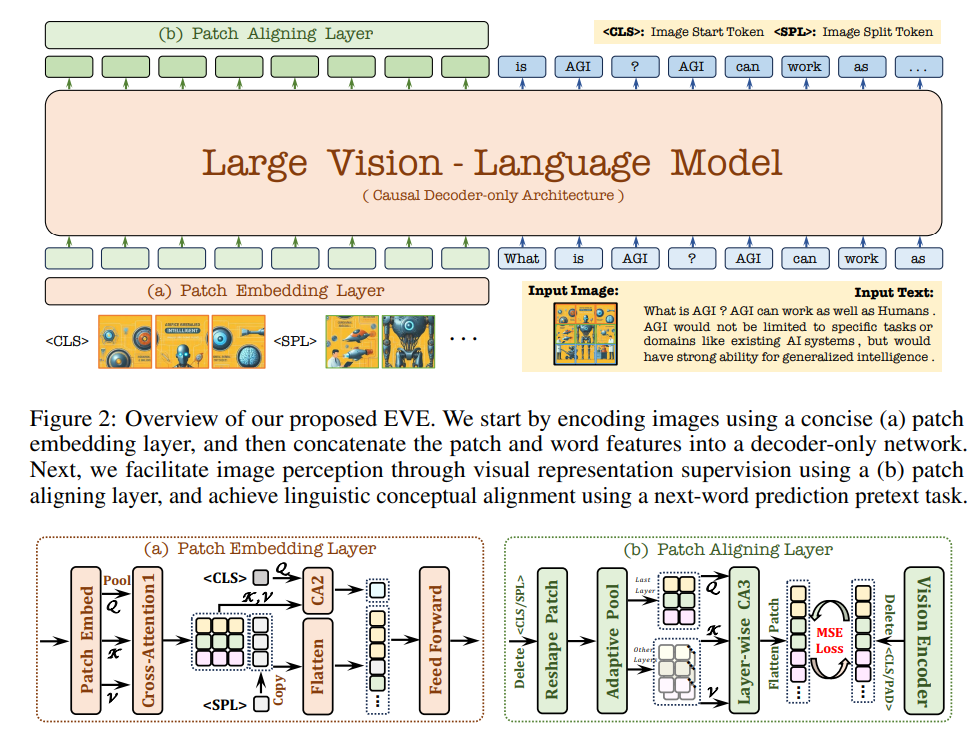
\includegraphics[width=1.0\textwidth]{images/lvlm_general_architecture.png}
	\captionof{figure}{Sơ đồ kiến trúc chung của một LVLM. Một Vision Encoder trích xuất đặc trưng từ ảnh. Một Module Kết nối ánh xạ các đặc trưng này vào không gian của LLM, cho phép LLM "nhìn thấy" và lý luận về ảnh.}
	\label{fig:lvlm_architecture}
\end{center}
% Keyword gợi ý: lvlm architecture, large vision language model diagram

\subsection{LLaVA (2023): Dân chủ hóa Nghiên cứu LVLM}
\label{subsec:llava}
\textbf{Large Language and Vision Assistant (LLaVA)} \cite{Liu2023_LLaVA} là một trong những dự án LVLM mã nguồn mở có ảnh hưởng nhất, chứng minh rằng có thể xây dựng các trợ lý thị giác mạnh mẽ mà không cần đến nguồn lực tính toán khổng lồ của các tập đoàn lớn.

\textbf{Kiến trúc và Phương pháp Huấn luyện:}
\begin{itemize}
	\item \textbf{Kiến trúc:} LLaVA tuân thủ nghiêm ngặt kiến trúc chung, kết hợp một Vision Encoder CLIP đã được đóng băng với một LLM mã nguồn mở (ban đầu là Vicuna, một biến thể của LLaMA). Module Kết nối chỉ là một lớp chiếu tuyến tính đơn giản.
	\item \textbf{Huấn luyện Hiệu quả:} Quá trình huấn luyện bao gồm hai giai đoạn:
	\begin{enumerate}
		\item \textbf{Pre-training for Alignment:} Huấn luyện chỉ Module Kết nối trên một bộ dữ liệu lớn các cặp (ảnh, chú thích) để học cách "dịch" các đặc trưng thị giác thành các "từ" mà LLM có thể hiểu.
		\item \textbf{Instruction Fine-tuning:} Tinh chỉnh cả Module Kết nối và LLM trên một bộ dữ liệu nhỏ hơn nhưng chất lượng cao hơn, bao gồm các hướng dẫn đa dạng (câu hỏi, mô tả, yêu cầu lý luận). Các tác giả đã sử dụng GPT-4 để tự động tạo ra bộ dữ liệu này.
	\end{enumerate}
\end{itemize}
\textbf{Tầm quan trọng:} LLaVA đã chứng minh rằng chỉ cần tinh chỉnh hiệu quả, một kiến trúc đơn giản có thể đạt được khả năng đối thoại và lý luận đa phương thức ấn tượng. Sự thành công và tính mở của nó đã thúc đẩy một làn sóng nghiên cứu khổng lồ, với nhiều biến thể như LLaVA-Next, VILA,...

\subsection{Gemini (Google DeepMind, 2023)}
\label{subsec:gemini}
\textbf{Gemini} \cite{GeminiTeam2023} là câu trả lời của Google cho GPT-4, được thiết kế ngay từ đầu như một mô hình \textbf{đa phương thức tự nhiên (natively multimodal)}.

\textbf{Triết lý Thiết kế:}
Thay vì "ghép" một vision encoder vào một LLM, Gemini được huấn luyện từ đầu trên một bộ dữ liệu khổng lồ bao gồm cả văn bản, hình ảnh, âm thanh và video được đan xen với nhau. Điều này cho phép nó học được các biểu diễn đa phương thức sâu sắc hơn và có khả năng lý luận phức tạp hơn trên nhiều loại dữ liệu.
\begin{itemize}
	\item \textbf{Khả năng Lý luận Tinh vi:} Gemini thể hiện khả năng vượt trội trong các benchmark đòi hỏi lý luận đa bước, chẳng hạn như giải các bài toán vật lý từ một bản vẽ tay, hoặc phân tích các biểu đồ khoa học phức tạp.
	\item \textbf{Hiểu biết Video và Âm thanh:} Khả năng xử lý video và âm thanh một cách tự nhiên là một điểm khác biệt lớn, cho phép Gemini hiểu được các chuỗi sự kiện và các tín hiệu động.
\end{itemize}
Gemini đại diện cho một thế hệ LVLM được xây dựng với tư duy "multimodal-first", hứa hẹn khả năng tương tác và thấu hiểu ở một cấp độ mới.

\subsection{GPT-4o (OpenAI, 2024): Hướng tới Tương tác Tức thời}
\label{subsec:gpt4o}
\textbf{GPT-4o} ("o" for "omni") \cite{OpenAI2024_GPT4o} là bước tiến mới nhất của OpenAI, tập trung vào việc tạo ra một trải nghiệm tương tác đa phương thức \textbf{tự nhiên và tức thời}.

\textbf{Đột phá Kỹ thuật:}
Trước GPT-4o, các hệ thống chatbot giọng nói đa phương thức thường bao gồm một pipeline gồm nhiều mô hình riêng biệt: một mô hình chuyển giọng nói thành văn bản, một mô hình xử lý văn bản và hình ảnh (như GPT-4V), và một mô hình chuyển văn bản thành giọng nói. Pipeline này tạo ra độ trễ lớn và làm mất mát thông tin (ví dụ: ngữ điệu, cảm xúc).

GPT-4o đã hợp nhất tất cả các thành phần này vào \textbf{một mô hình end-to-end duy nhất}.
\begin{itemize}
	\item Nó có thể nhận đầu vào là bất kỳ sự kết hợp nào của văn bản, âm thanh, và hình ảnh, và tạo ra đầu ra cũng dưới dạng kết hợp của chúng.
	\item \textbf{Tốc độ Phản hồi:} Bằng cách loại bỏ pipeline phức tạp, GPT-4o có thể phản hồi các đầu vào âm thanh và hình ảnh với độ trễ chỉ vài trăm mili giây, gần với tốc độ phản ứng của con người.
	\item \textbf{Hiểu biết Ngữ điệu và Cảm xúc:} Vì xử lý âm thanh một cách trực tiếp, GPT-4o có thể nhận biết được các sắc thái trong giọng nói như cảm xúc, tiếng cười, và có thể tạo ra giọng nói với các ngữ điệu khác nhau.
\end{itemize}
GPT-4o đã đặt ra một tiêu chuẩn mới về sự tự nhiên và tốc độ trong tương tác người-máy đa phương thức, biến LVLMs từ các công cụ phân tích thành các "trợ lý AI" có khả năng đối thoại thực sự.

\subsection{Kết luận: Kỷ nguyên của các Trợ lý Thị giác}
\label{subsec:lvlm_conclusion}
LVLMs như LLaVA, Gemini, và GPT-4o đang định nghĩa lại ranh giới của thị giác máy tính. Chúng đã biến đổi các mô hình từ những công cụ nhận dạng thụ động thành các tác nhân (agents) có khả năng tương tác, lý luận và giao tiếp về thế giới thị giác.

Sự phát triển nhanh chóng trong lĩnh vực này cho thấy một tương lai nơi các hệ thống AI sẽ không còn bị giới hạn bởi một phương thức duy nhất. Chúng sẽ có khả năng tích hợp thông tin từ tất cả các giác quan kỹ thuật số để xây dựng một sự hiểu biết toàn diện và sâu sắc về thế giới—một bước tiến quan trọng trên con đường hướng tới trí tuệ nhân tạo tổng quát.

\section*{Tài liệu tham khảo}
\begin{itemize}
	\item[1] Liu, H., Li, C., Wu, Q., \& Lee, Y. J. (2023). Visual instruction tuning. In \textit{Advances in Neural Information Processing Systems (NeurIPS)}. (Paper gốc giới thiệu LLaVA).
	\item[2] Gemini Team. (2023). Gemini: A family of highly capable multimodal models. \textit{arXiv preprint arXiv:2312.11805}. (Báo cáo kỹ thuật giới thiệu họ mô hình Gemini).
	\item[3] OpenAI. (2024). \textit{GPT-4o Technical Report}. OpenAI Blog and System Card. (Công bố và phân tích về GPT-4o).
	\item[4] OpenAI. (2023). \textit{GPT-4V(ision) System Card}. (Báo cáo về phiên bản GPT-4 có khả năng xử lý hình ảnh, tiền thân của GPT-4o).
	\item[5] Radford, A., Kim, J. W., Hallacy, C., Ramesh, A., Goh, G., Agarwal, S., ... \& Sutskever, I. (2021). Learning transferable visual models from natural language supervision. In \textit{International Conference on Machine Learning (ICML)}. (Paper về CLIP, công nghệ nền tảng cho nhiều LVLMs).
	\item[6] Alayrac, J. B., et al. (2022). Flamingo: a visual language model for few-shot learning. In \textit{Advances in Neural Information Processing Systems (NeurIPS)}. (Một LVLM quan trọng khác, tập trung vào khả năng few-shot learning).
\end{itemize}